\chapter{Исследовательский раздел}
В данном разделе проведено исследование разработанной программы.

Исследования проводились на машине со следующими характеристиками:
\begin{itemize}[label=---]
	\item процессор Intel(R) Core(TM) i5-10210U, тактовая частота 1.60 ГГц;
	\item оперативная память: 16 ГБ;
	\item операционная система: Ubuntu 22.04.4 LTS.
\end{itemize}

\section{Цель исследования}

Размер ограничивающего столб пепла параллелепипеда и, как следствие, число вокселей напрямую влияет на производительность симуляции. Большинство методов расчета движения газа имеют кубическую сложность. Метод решения СЛАУ также дополнительно требует провести несколько итераций вычисления каждого неизвестного. Для увеличения производительности предлагается~\cite{norway} использование параллельных вычислений.

Цель исследования --- определить какую долю от общего времени выполнения алгоритма, занимают основные его части, для дальнейшего распараллеливания вычислений.

\section{Исследование}

Для исследования выделены основные части в алгоритме основанном на уравнениях Навье---Стокса:
\begin{itemize}
	\item добавление источника дыма;
	\item решение СЛАУ для вычисления диффузии дыма;
	\item адвекция дыма;
	\item добавление источников скорости;
	\item решение СЛАУ для вычисления рассеивания скорости;
	\item самоадвекция скорости.
\end{itemize}

Для выполнения исследования, были проведены замеры времени основных этапов алгоритма для генерации 1000 кадров. Полученные результаты представлены в таблице~\ref{tab:no_parallel}.

\begin{table}[H]
	\caption{Распределение времени выполнения этапов алгоритма генерации дыма}
	\label{tab:no_parallel}
	\centering
	\begin{tabular}{|c|c|c|}
		\hline
		Этап&\shortstack{Доля от общего\\времени выполнения (\%)}&\shortstack{Среднее время\\ выполнения (сек)}\\\hline
		Добавление источников дыма&0.98&0.003\\\hline
		Решение СЛАУ для диффузии &70.26&0.214\\\hline
		Адвекция дыма&19.94&0.061\\\hline
		Добавление источников скорости&0.28&0.001\\\hline
		Решение СЛАУ для рассеивания скорости&22.49&0.068\\\hline
		Самоадвекция скорости&8.55&0.026\\\hline\hline
		Сумма&100&	0.372\\\hline
	\end{tabular}
\end{table}

На рисунке~\ref{fig:no_parallel} приведены результаты исследования в виде круговой диаграммы.

\begin{figure}[H]
	\centering
	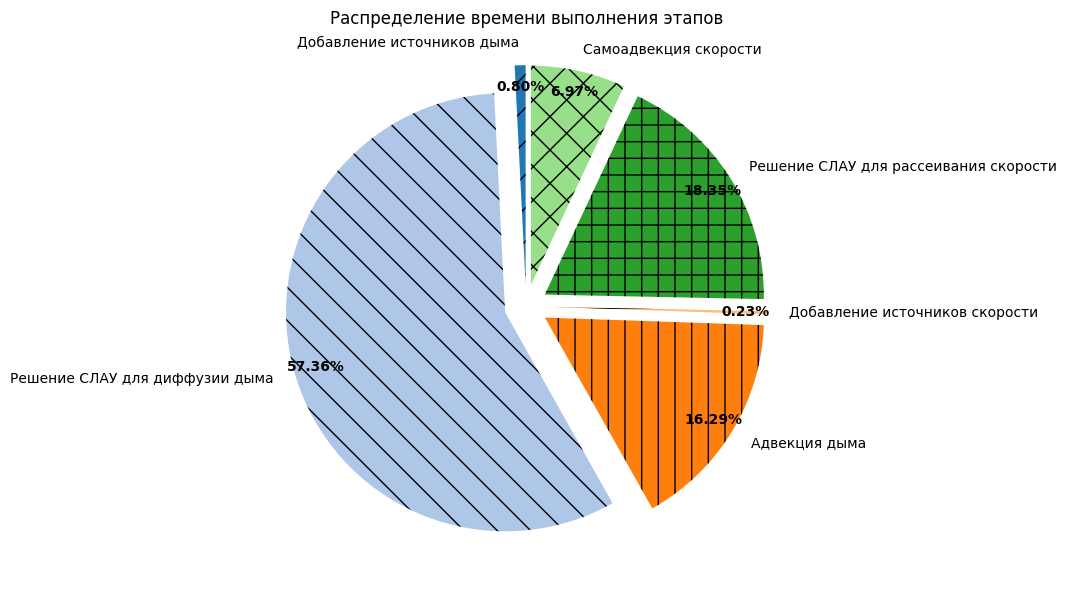
\includegraphics[width=1.0\textwidth,page=1]{assets/img/pie.png}
	\caption{Диаграмма распределения времени выполнения этапов алгоритма генерации дыма}
	\label{fig:no_parallel}
\end{figure}

Для проверки полученных результатов, были проведены аналогичные замеры для тех же этапов с использованием параллельных вычислений. Для обеспечения параллельности была использована библиотеки OpenMP~\cite{OpenMP}. Полученные результаты представлены в таблице~\ref{tab:parallel} и на рисунке~\ref{fig:parallel}.

\begin{table}[H]
	\caption{Распределение времени выполнения этапов алгоритма генерации дыма при использовании параллельных вычислений}
	\label{tab:parallel}
	\centering
	\begin{tabular}{|c|c|c|}
		\hline
		Этап&\shortstack{Доля от общего\\времени выполнения (\%)}&\shortstack{Среднее время\\ выполнения (сек)}\\\hline
		Добавление источников дыма&1.99&0.004\\\hline
		Решение СЛАУ для диффузии &57.14&0.106\\\hline
		Адвекция дыма&11.68&0.022\\\hline
		Добавление источников скорости&0.56&0.001\\\hline
		Решение СЛАУ для рассеивания скорости&22.49&0.041\\\hline
		Самоадвекция скорости&6.14&0.011\\\hline\hline
		Сумма&100&	0.185\\\hline
	\end{tabular}
\end{table}

\begin{figure}[H]
	\centering
	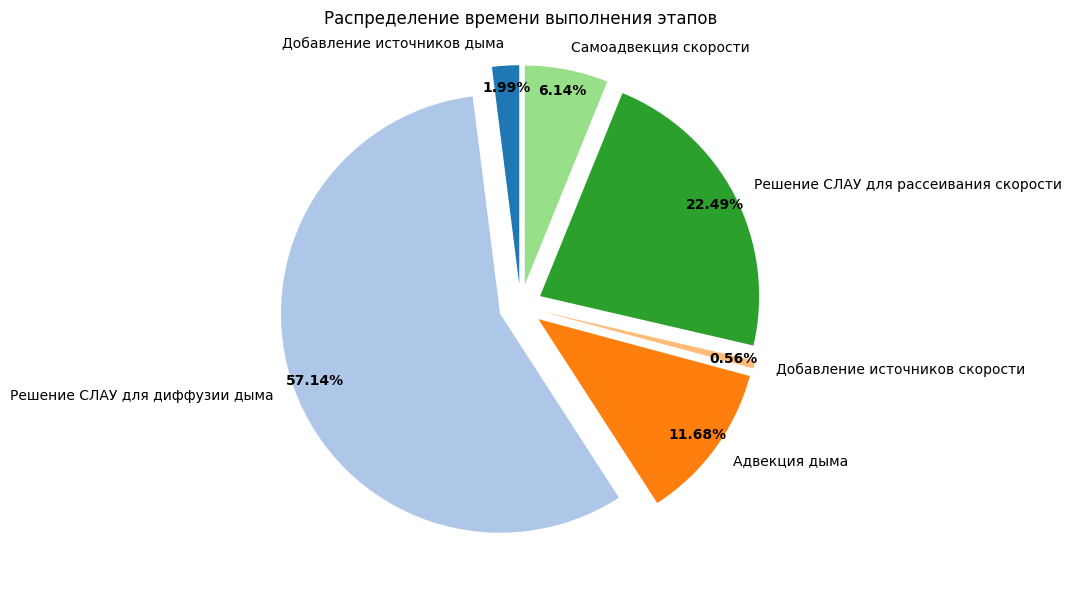
\includegraphics[width=1.0\textwidth,page=1]{assets/img/pie_parallel.png}
	\caption{Диаграмма распределения времени выполнения этапов алгоритма генерации дыма с использованием параллельных вычислений}
	\label{fig:parallel}
\end{figure}

\section*{Вывод}
В данной части была описана цель исследования, технические характеристики устройства, были приведены результаты исследования.

Была произведена серия экспериментов, в результате которых было вычислено среднее время визуализации и обновление физики для разного количества вокселей. Также был проведен опрос для выяснения оптимального количества пикселей для реалистичности воздействия ветра на сакуру. Оказалось, что большинство респондентов выбрали вариант с 5000 вокселей.
